\chapter{Top Features by Mutual Information}\label{app:mi}

\jh{threashold do zvl sloupecku}
\jh{Kratky komentar na zacatek - kde je o tom vic, kde je definovana MI, ...}
\jh{je k tomu nekde aspon minimalni komentar? Pokud ne, dejte ho sem "From the graph, we can see that a small number (..) of unigrams ...}
\jh{grafy - co je na ktere ose?, Jedna osa je logaritmicka, treba zminit}


\begin{table}[h!]

\centering
\begin{tabular}{lS[table-format=3.2]}
\toprule
\textbf{feature (threshold)} & \textbf{mutual information} \\
\midrule
error rate (0.02) & 0.00007 \\
error rate (0.05) & 0.00182 \\
error rate (0.1) & 0.00174 \\
error rate (0.15) & 0.00074 \\
error rate (0.2) & 0.00038 \\
error total (5) & 0.00000 \\
error total (10) & 0.00000 \\
error total (15) & 0.00000 \\
error total (20) & 0.00000 \\
\bottomrule
\end{tabular}

\caption{Mutual information of spelling mistakes}\label{tab:mi_errors}
\end{table}

\begin{table}[h!]

\centering
\begin{tabular}{lS[table-format=3.2]}
\toprule
\textbf{feature (threshold)} & \textbf{mutual information} \\
\midrule
biz stars (1, 2, 3, 4, 5) & 0.00112 \\
extreme stars (1, 5) & 0.00175 \\
stars (1, 2, 3, 4, 5)& 0.01060 \\
stars (1) & 0.00657 \\
stars (2) & 0.00204 \\
stars (3) & 0.00221 \\
stars (4) & 0.00137 \\
stars (5) & 0.00004 \\
\bottomrule
\end{tabular}

\caption{Mutual information of stars}\label{tab:mi_stars}
\end{table}

\begin{table}[h!]

\centering
\begin{tabular}{lS[table-format=3.2]}
\toprule
\textbf{feature (threshold)} & \textbf{mutual information} \\
\midrule
review length (50, 150) & 0.07866 \\
review length (35) & 0.02680 \\
review length (50) & 0.04091 \\
review length (75) & 0.05996 \\
review length (100) & 0.06726 \\
review length (150) & 0.06580 \\

\bottomrule
\end{tabular}
\caption{Mutual information of the number of words}\label{tab:mi_words}
\end{table}

\begin{table}[h!]
\centering
\begin{tabular}{lS[table-format=3.2]}
\toprule
\textbf{feature (threshold)} & \textbf{mutual information} \\
\midrule
sentiment (neg, neut, pos) & 0.00969 \\
\bottomrule
\end{tabular}
\caption{Mutual information of sentiment}\label{tab:mi_sentiment}
\end{table}



\begin{table}[h!]
\centering
\begin{tabular}{lS[table-format=3.2]}
\toprule
\textbf{feature (threshold)} & \textbf{mutual information} \\
\midrule
instance 1 (0.4) & 0.00006 \\
instance 1 (0.6) & 0.00002 \\
instance 1 (0.8) & 0.00002 \\
instance 1 (0.9) & 0.00002 \\
instance 1 (0.95) & 0.00002 \\
instance 2 (0.4) & 0.00004 \\
instance 2 (0.6) & 0.00002 \\
instance 2 (0.8) & 0.00002 \\
instance 2 (0.9) & 0.00002 \\
instance 2 (0.95) & 0.00002 \\
\bottomrule
\end{tabular}
\caption{Mutual information of cosine similarity (2 best performing instances)}\label{tab:mi_cossim}
\end{table}

\begin{figure}[ht]\centering
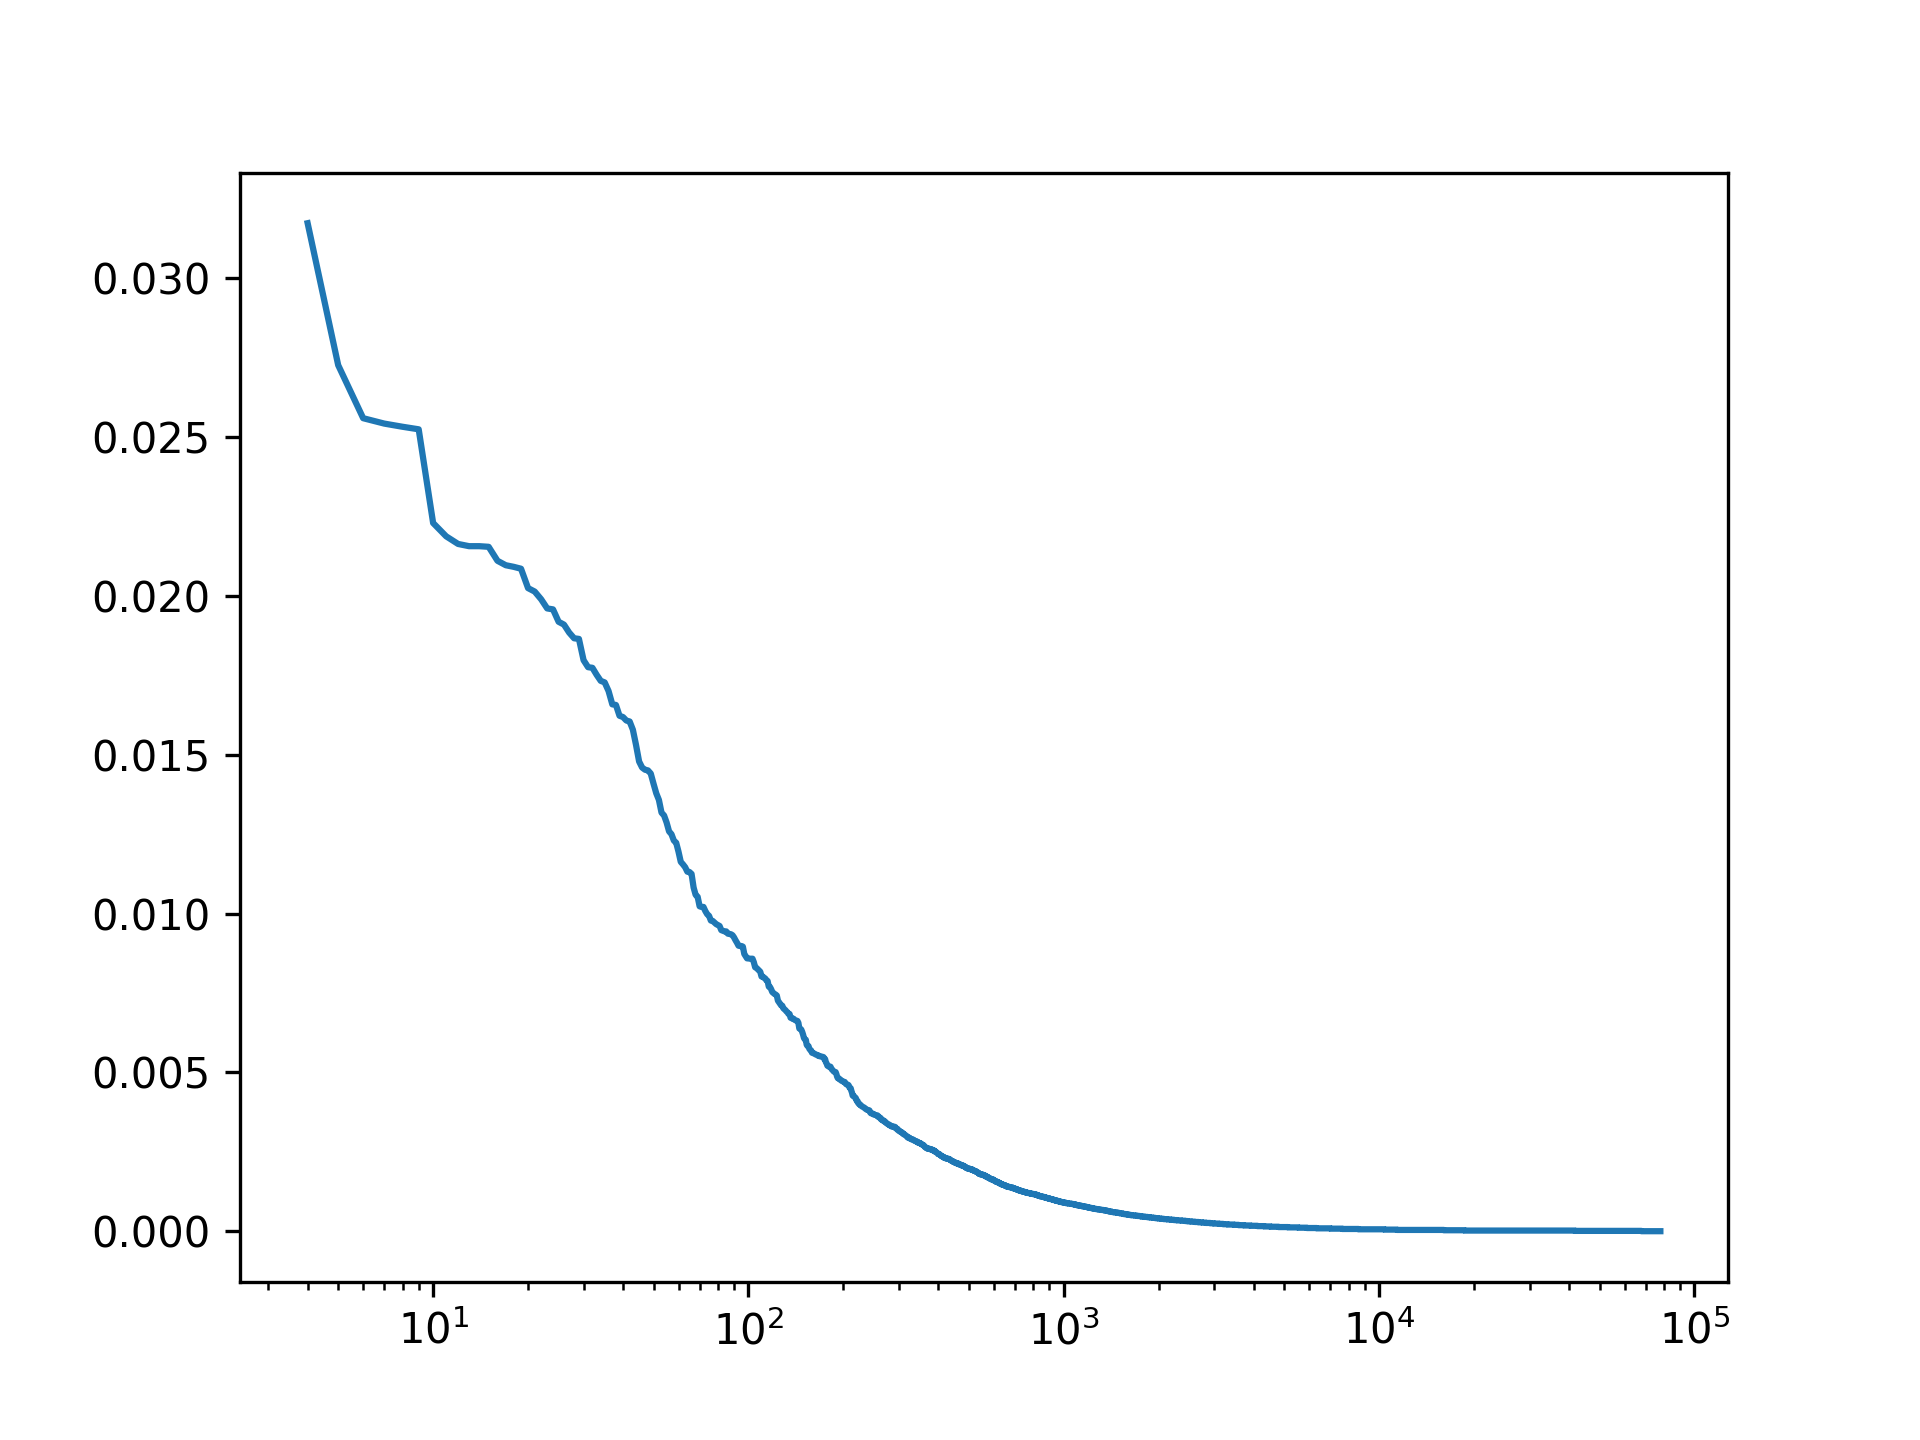
\includegraphics[width=130mm]{figures/unigrams.png}
\caption{Mutual information of unigrams}
\label{fig:mi_unigrams}
\end{figure}

\begin{figure}[ht]\centering
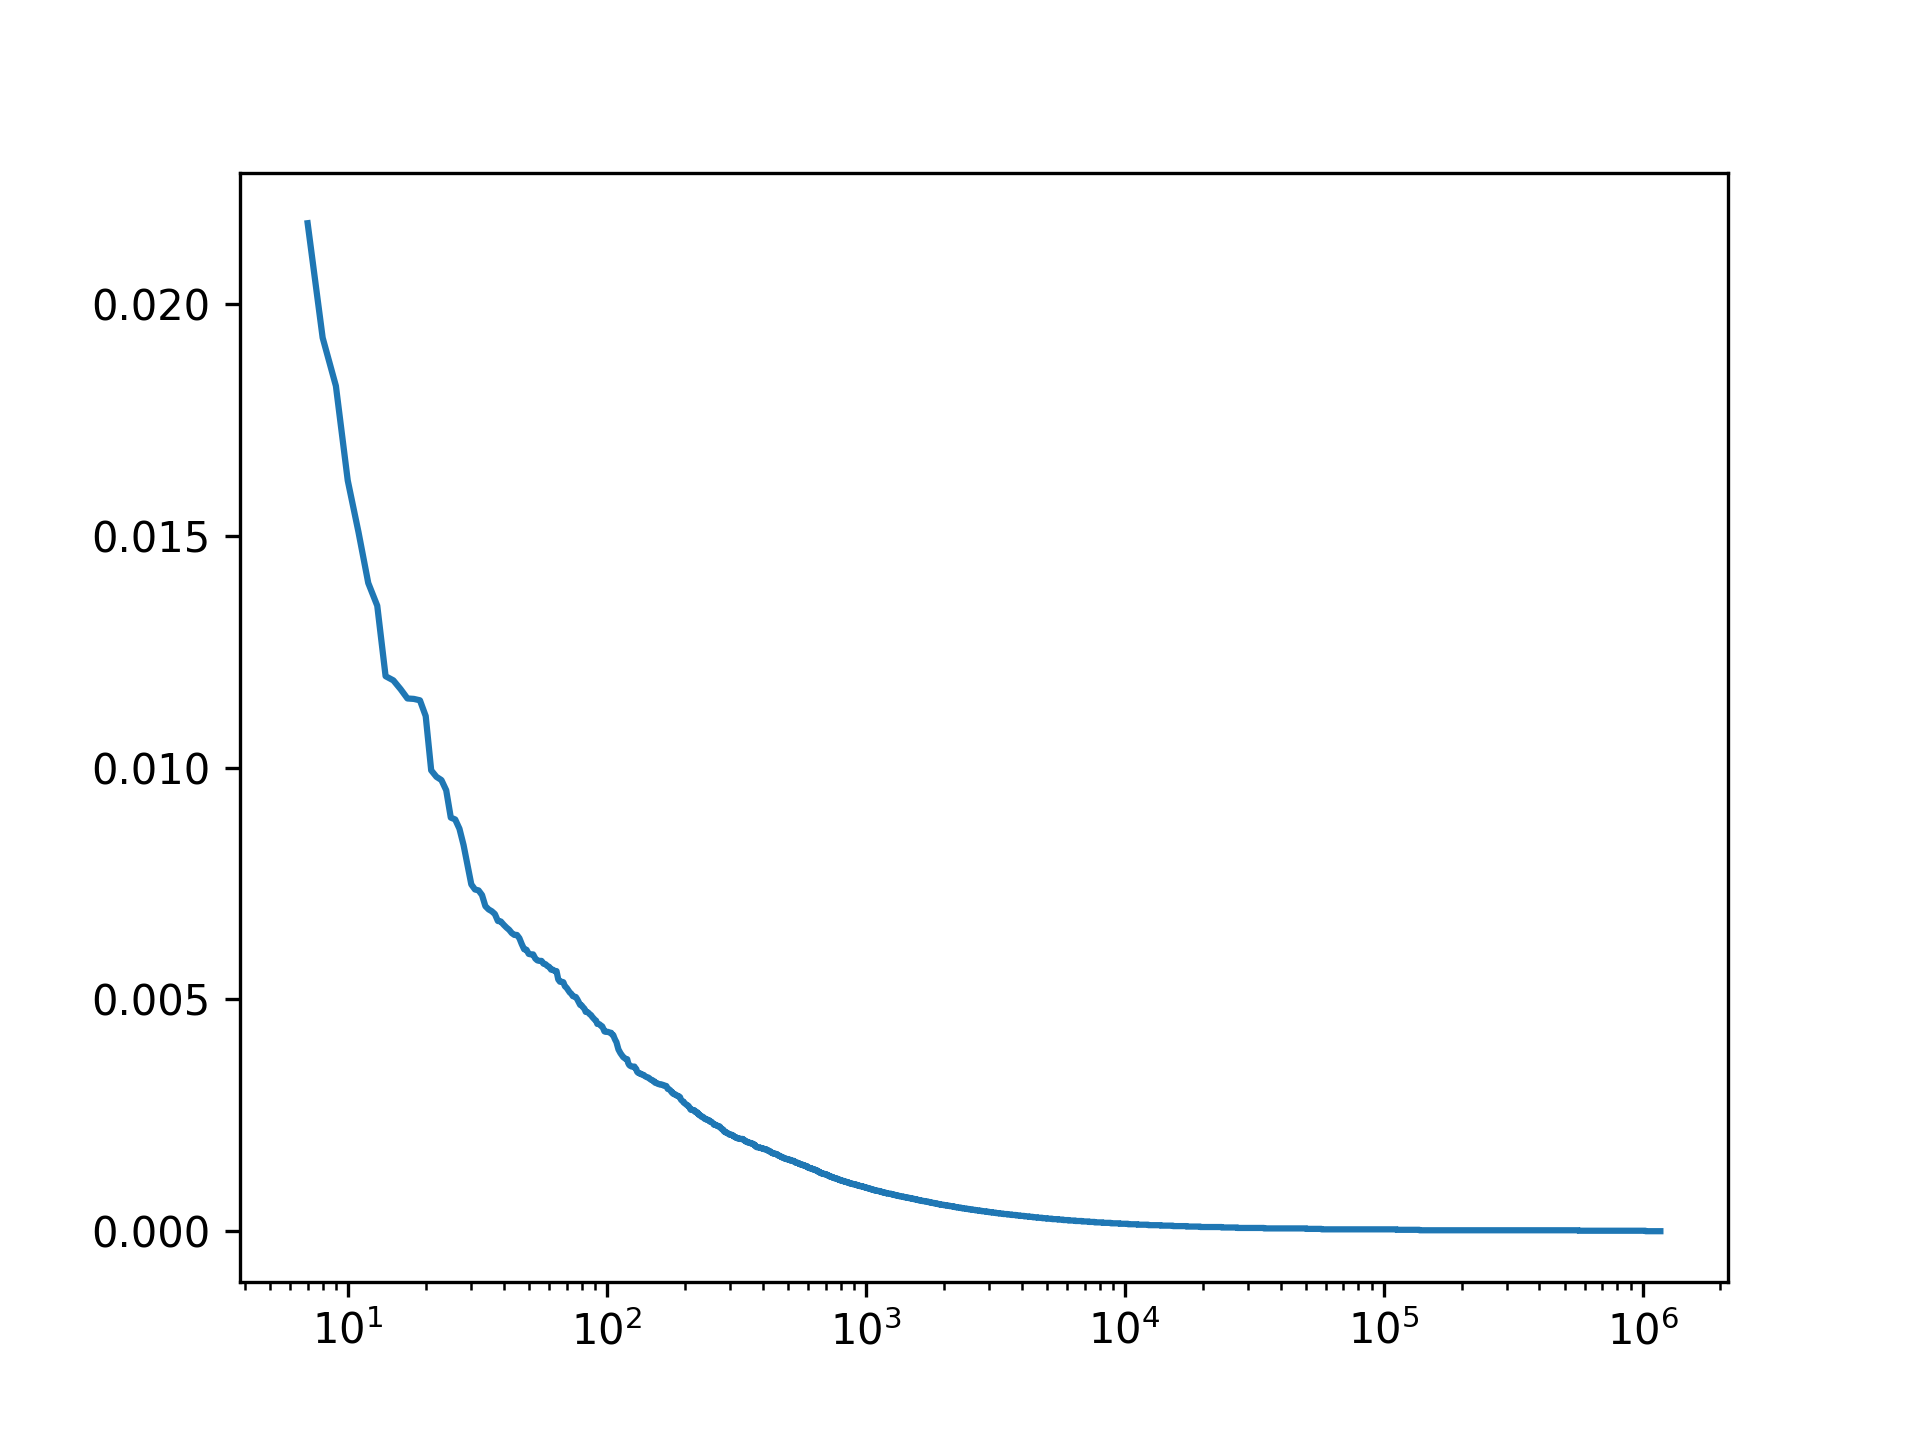
\includegraphics[width=130mm]{figures/bigrams.png}
\caption{Mutual information of bigrams}
\label{fig:mi_bigrams}
\end{figure}

\begin{figure}[ht]\centering
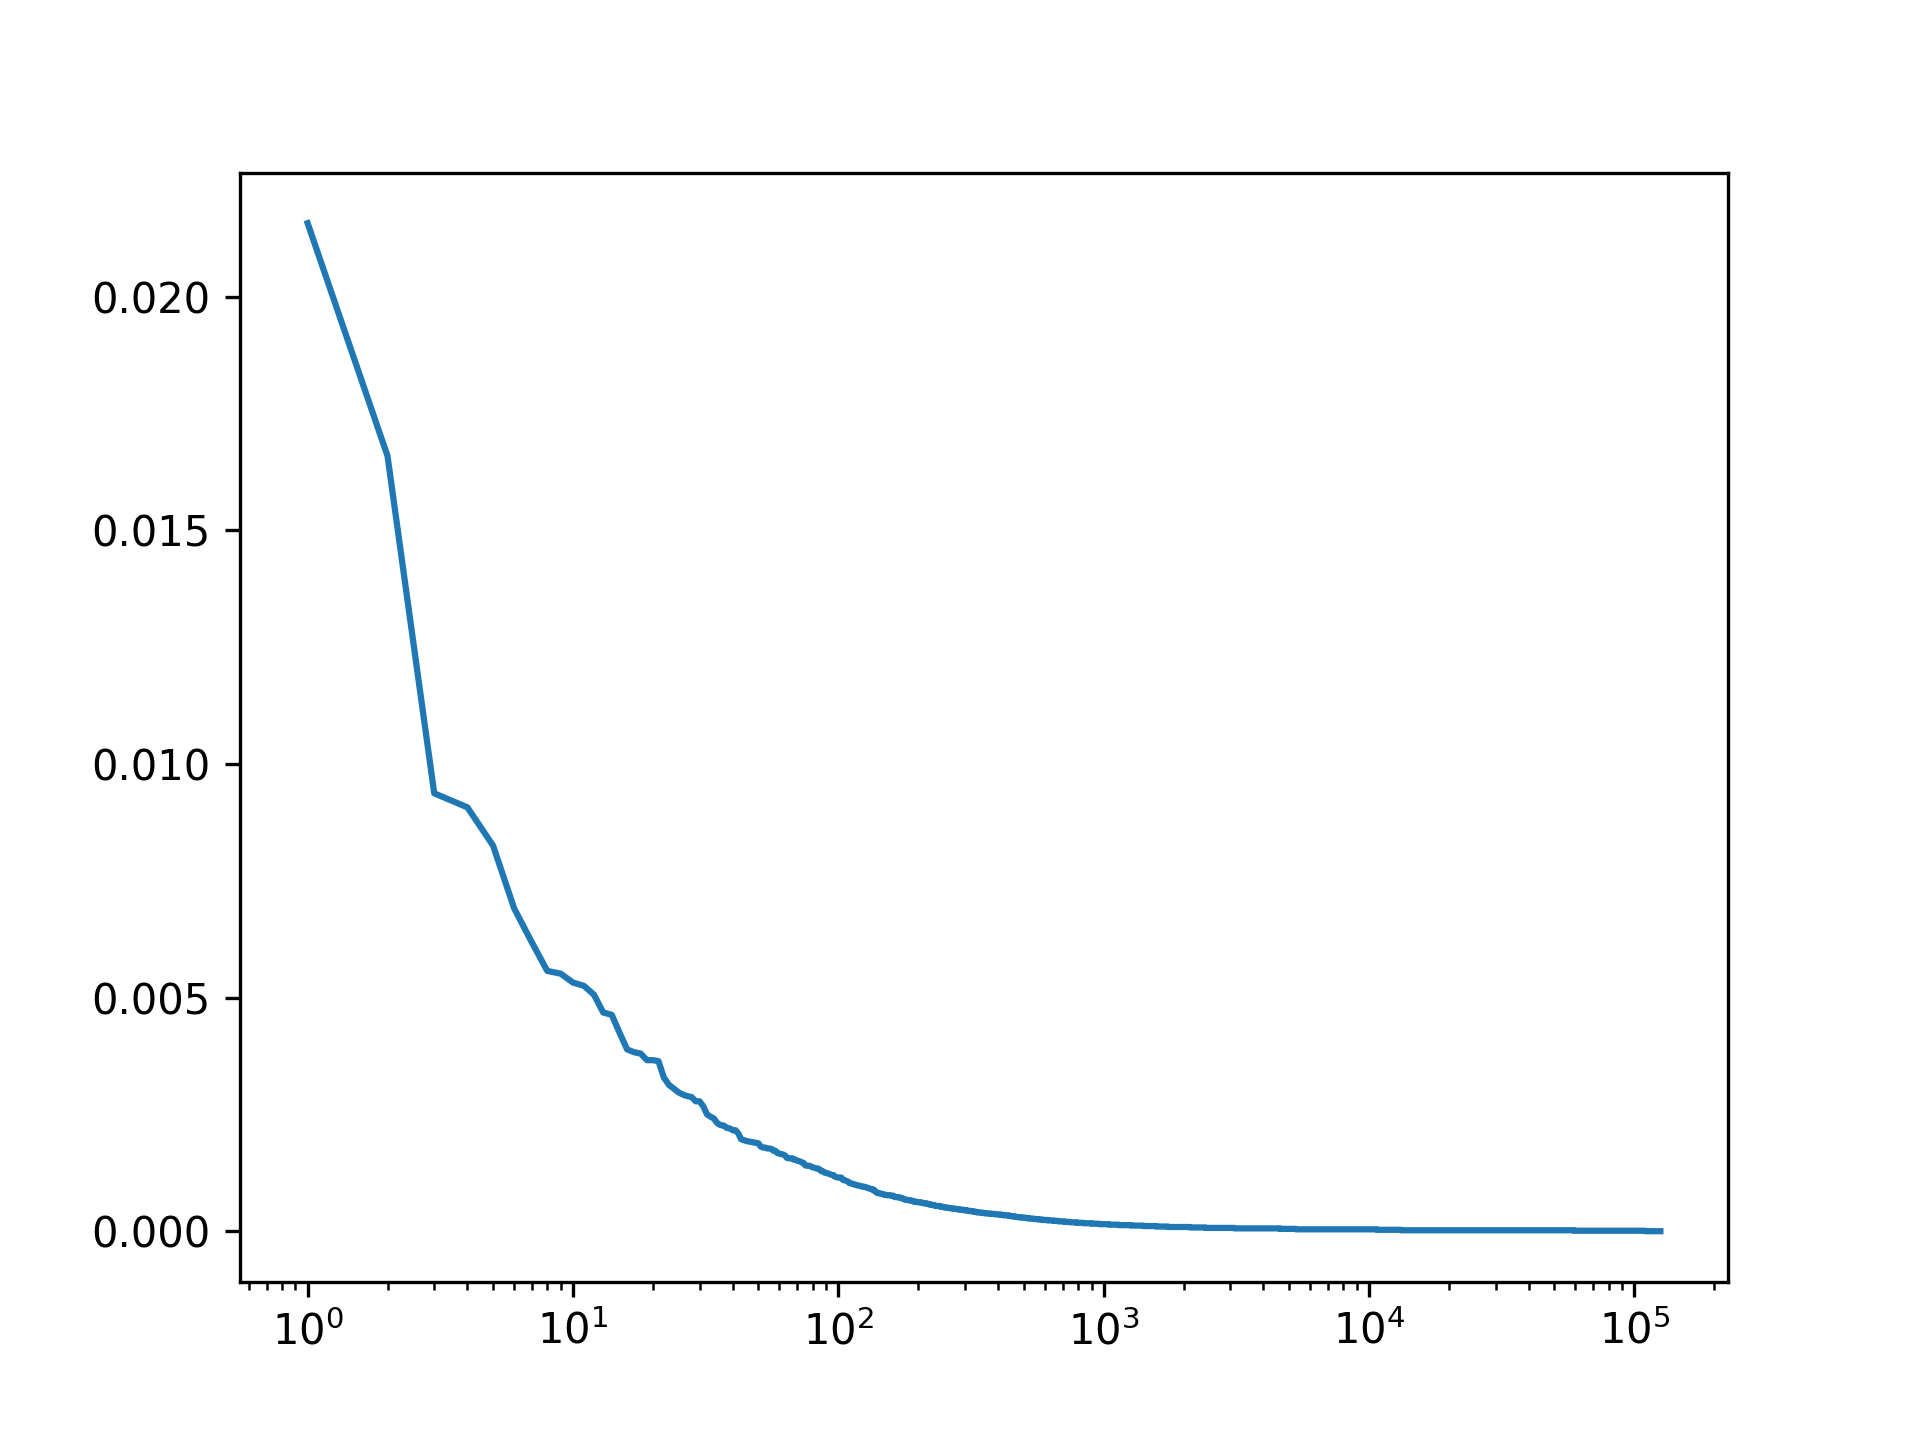
\includegraphics[width=130mm]{figures/entities.png}
\caption{Mutual information of entities}
\label{fig:mi_entities}
\end{figure}
